\documentclass[aps, twocolumn, secnumarabic, amsmath, amssymb, nofootinbib, floatfix]{revtex4-1}
\usepackage{graphicx, bm}
\usepackage[colorlinks=true]{hyperref}

\begin{document}
\title{Estimating Cube Volume by Hand Measurement}
\author{Henry Shackleton}
\email{hshackle@mit.edu}
\homepage{henryshackleton.com}
\date{\today}
\affiliation{MIT Depatment of Physics}

\begin{abstract}
  Using data collected over several years from 8.13 students measuring the volume of a cube, we analyze the data as a collection of measurements to obtain a more accurate volume estimate of $(3.4 \pm .01_\text{stat} \pm .19_\text{sys}) \times 10^3$ mm$^3$. The statistical uncertainty is derived from considering the standard deviation and number of counts in the volume distribution, whereas systematic uncertainty arises from reported uncertainty in individual measurements. This paper is written in response to Homework 2 of 8.13.
\end{abstract}

\maketitle
\begin{figure}
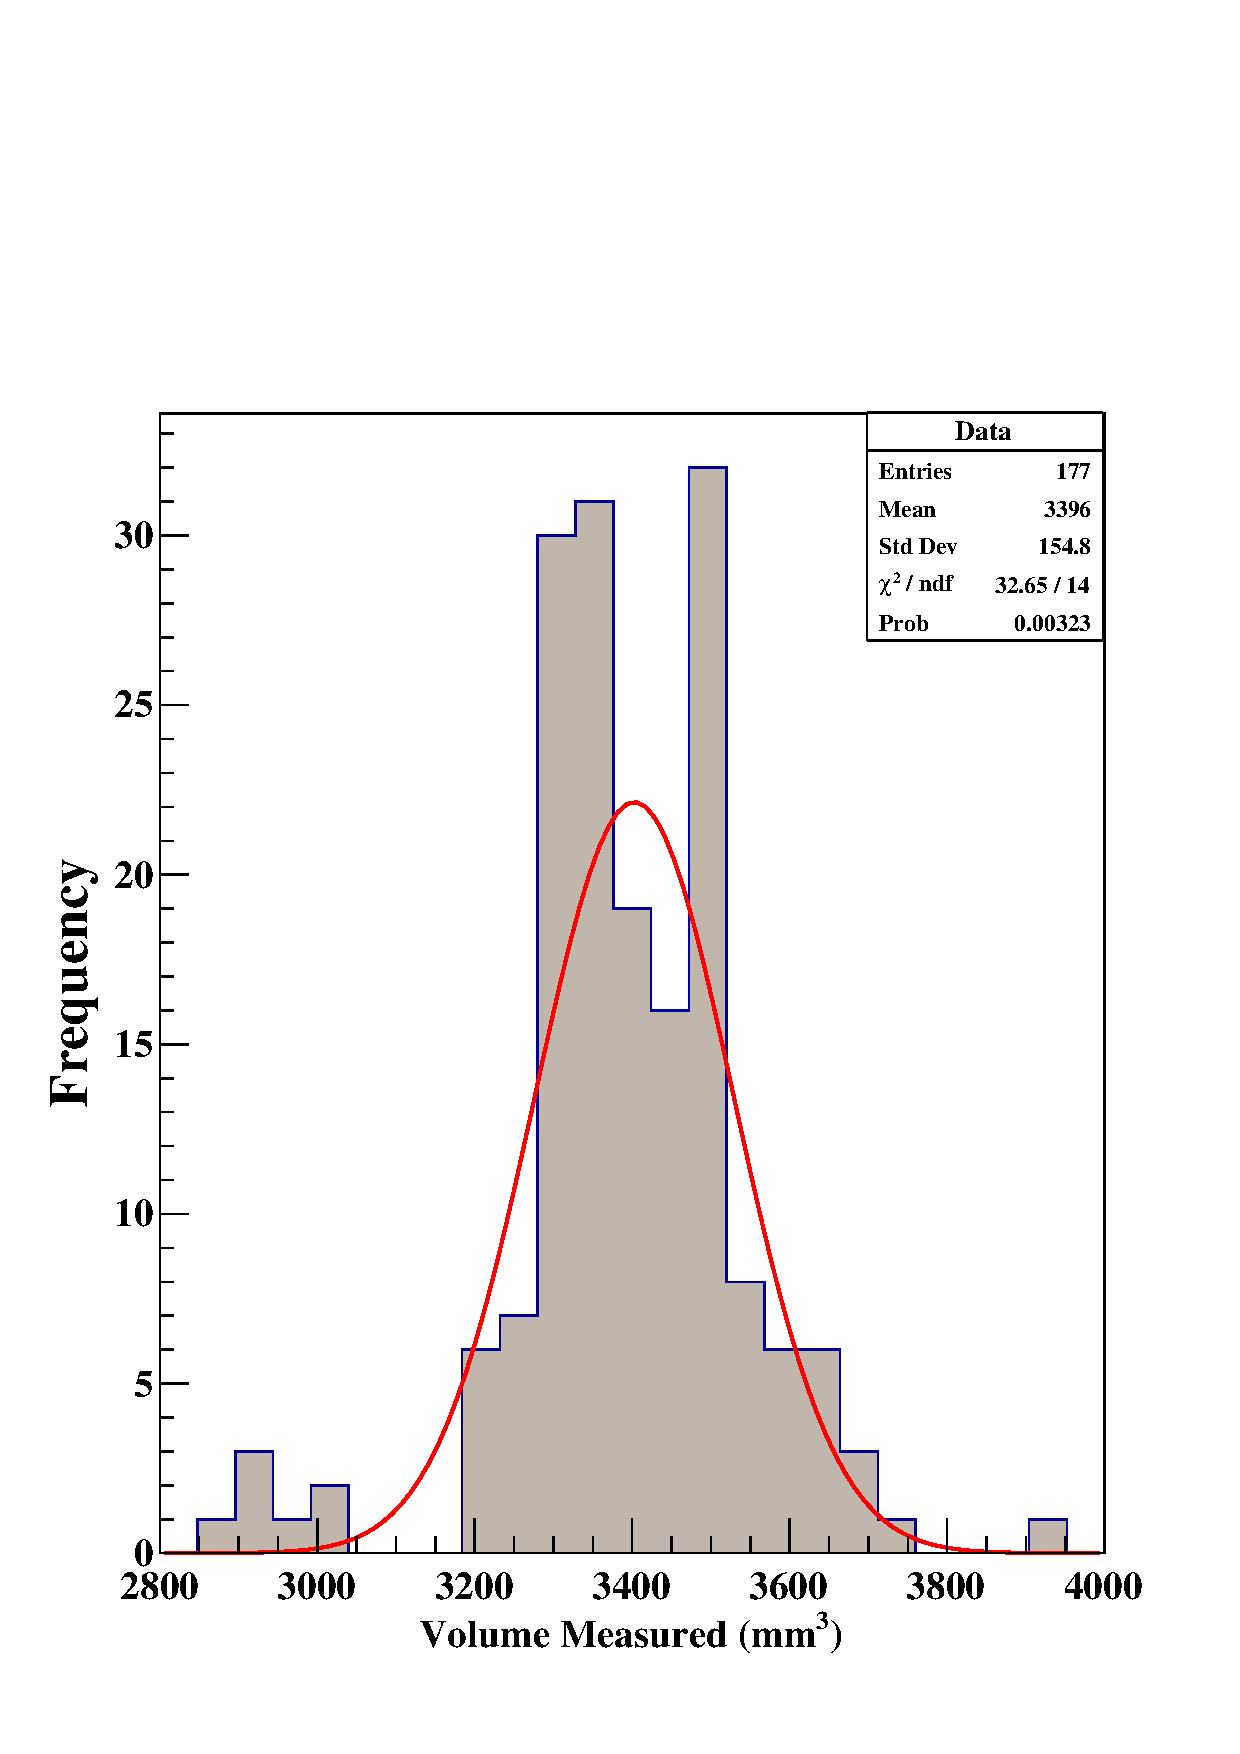
\includegraphics[width=8.6cm]{c1.pdf}
\caption{This histogram displays the distribution of 177 reported volumes of an aluminum cube, overlaid with a continuous Gaussian according to the mean and standard deviation of the distribution.}
  \end{figure}
As reported earlier, the systematic uncertainty in individual measurements was on average 192 mm$^3$, which means that the bin size of 24 mm is significantly smaller than the estimated uncertainty. However, the particularly large systematic uncertainty reported means that a bin size corresponding to it would lose most of the detail of the histogram. We have kept the bin sizes at 24 to more easily show trends in data reporting. Most notable are the three sharp peaks within the 3200 to 3600 mm$^3$ range, which correspond to reported length, width, and height at integers values. This suggests a bias in the measurements, in which people have a tendency to round up or down so as to report integers.
\end{document}
